\section{Anwendung des Kalman-Filters}
Bis jetzt haben wir gesehen, was das Kalman-Filter bewirkt und wie es funktioniert.
Nun möchten wir mit einem konkreten Beispiel herausfinden,
ob das Filter unsere gesuchte Grösse $f(t)$ bestimmen kann.

Da wir keine Rohdaten über vergangene Erdbeben zur Hand haben,
müssen wir mittels Simulation künstliche Daten erzeugen.
Diese können wir dann mit unserem Filter verarbeiten.
Diese Vorgehensweise erlaubt uns das Erdbeben beliebig zu gestalten
und weil es digital simuliert wird, haben wir auch keine Bauschäden zu beklagen.

\subsection{Wahl der Schwingung}
Wir müssen uns überlegen, mit welcher Schwingung wir ein realitätsnahes Beben erzeugen können.
Mit einer ungedämpften harmonischen Schwingung können wir zwar die meisten Vorgänge in der Physik erklären.
Da ein Erdbeben vorteilhafterweise irgendwann abklingen sollte,
wählen wir eine gedämpfte harmonische Schwingung
\begin{equation}
  y = A e^{-\lambda t} \sin(2\pi f t).
\end{equation}

In unsere Simulation können wir die Parameter frei wählen.
Wir setzten $A = 5$ für die Amplitude der Schwingung.
Sie beschreibt die Heftigkeit des Erdebebens und ist vergleichbar mit der Magnitude.

Für die Frequenz $f$ wählen wir eine Zufallssquenz mit Erwartungswert und Standardabweichung
\begin{equation}
  \mu = \SI{15}{\hertz}
  \qquad\text{und}\qquad
  \sigma = \SI{10}{\hertz}.
\end{equation}
Zusätzlich haben wir $f$ mit einem Savitzky-Golay-Filter gefiltert.
Ein Savitzky-Golay-Filter schaut sich immer eine definierte Anzahl von Datenpunkte an
und bildet ein Polynom $n$-ter Ordnung.
In unserer Anwendung schaut sich das Filter, im Sinne eines verschiebbaren Fensters,
jeweils elf aufeinanderfolgende Datenpunkte an und bildet ein Polynom $0$-ter Ordnung,
also eine Konstante.
Somit erhalten wir mit Matlab-Standardfunktionen einen gleitenden Mittelwert,
um all zu schnelle Änderungen der Frequenz zu unterdrücken.

$\lambda$ ist die Bodendämpfung, für die wir $0.2$ wählen.
Sie ist dafür verantwortlich, dass unser Erdbeben abklingt
und kreiert bei der gedämpften Schwingung die typische Hüllkurve.
Wir nehmen an, dass $\lambda$ ein Materialparameter von geologischen Böden ist.

\subsection{Versuch im Standardfall}
Im nächsten Schritt müssen wir sinnvolle Systemparameter für unseren Seismographen definieren.
Eine kurze Recherche zeigt, dass die Masse ein Gewicht von ca.\ \SI{100}{\gram} hat.
Zur Federkonstante $D$ und Dämpfung $k$ konnten wir leider keine brauchbaren Grössen finden.
Wir treffen die Annahmen $D = 1$ und $k = 0.01$.
Für die Masse definieren wir $m = 0.01$.

Für das Prozessrauschen werden die Bedingungen
\begin{equation}
  Q = 
  \begin{pmatrix}
    \sigma_x ^2 & 0          & 0 \\
    0           & \sigma_v^2 & 0\\
    0           & 0          & \sigma_f^2 \\
  \end{pmatrix}=
  \begin{pmatrix}
    0.00001^2& 0& 0 \\
    0 & 0.00001^2& 0\\
    0 & 0& 1^2 \\
  \end{pmatrix}
\end{equation}
angesetzt.
Die Annahme, dass sich die Erdbebenkraft $F$ nicht ändert,
kompensieren wir hier endlich durch einen grossen Wert von $\sigma_F^2$.
Auch für die Messung setzen wir ein Rauschen voraus und definieren
\begin{equation}
  R
  = 
  ( \sigma_x^2 )
  =
  (0.00001^2)
  .
\end{equation}
Damit sind nun die benötigten Systemparameter und das Rauschen definiert.
Als nächstes erzeugen wir ein Erdbeben und schauen,
wie gut das Kalman-Filter die äussere Beschleunigung schätzen kann.

\subsection*{Ergebnis}

Wie wir in Abbildung~\ref{erdbeben:fig:standard-alles} im Positions-Zeit-Diagramm sehen, erzeugen unsere vorher gewählten Parameter eine realistische Erdbebenaufzeichnung.
Leiten wir die Position einmal ab, erhalten wir die Geschwindigkeit.
Die zweite Ableitung ergibt uns die Kraft, die in unserer Aufgabenstellung gesucht ist.

Zoomen wir näher ran, erkennen wir wieder im Positions-Diagramm eine Überlagerung der Massen-Eigenschwingung mit der Erdbebenschwingung.
Die Masse schwingt mit einer tiefen Frequenz und hoher Amplitude, hingegen das Erdbeben mit einer hohen Frequenz und tiefer Amplitude.

Vergleichen wir nun die Position mit der Kraft, stellen wir fest, dass das Kalman-Filter eine Schätzung wiedergibt, die auch eine Frequenz von \SI{15}{\hertz} hat.
Das Filter war imstande die Eigenfrequenz zu eliminieren und die tatsächliche Kraft des Erdbebens wiederzugeben.

\begin{figure}
  \begin{center}
    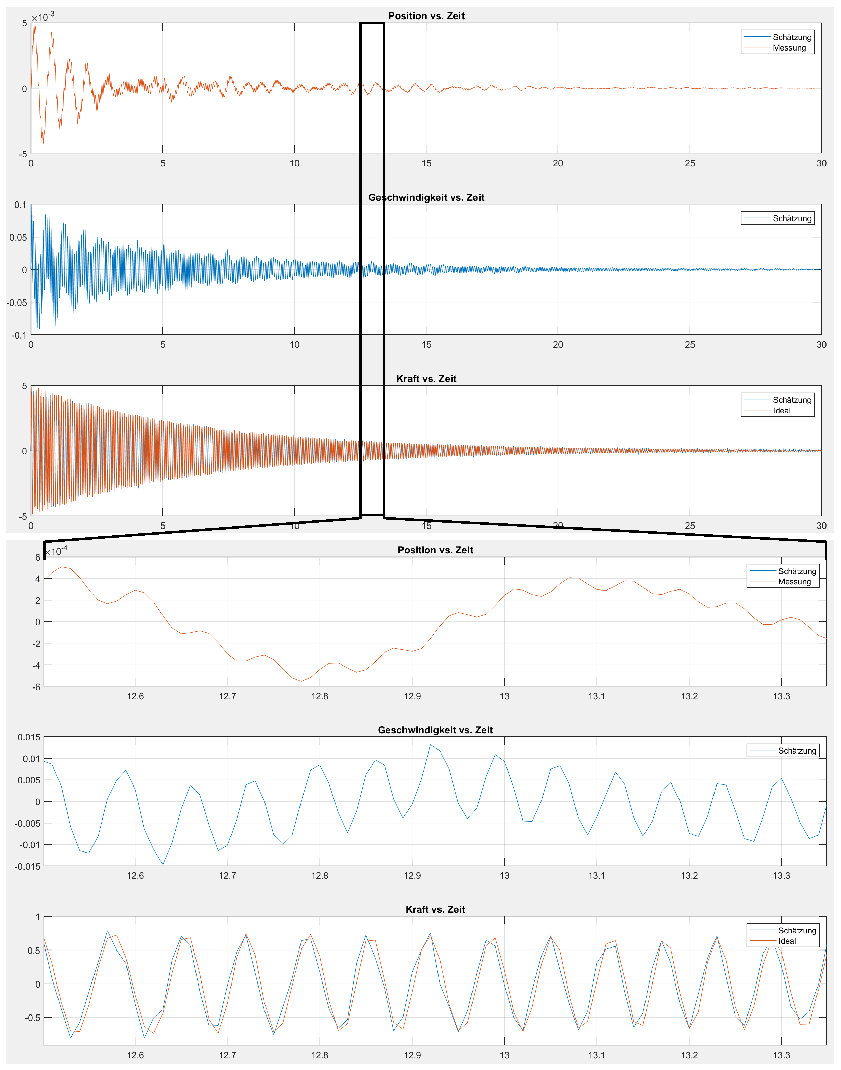
\includegraphics[width=.95\linewidth,keepaspectratio]{papers/erdbeben/images/standard.PDF}
    \caption{
      Das Position-Zeit-Diagramm zeigt eine typische Aufzeichnung eines Seismographen während eines Erdbebens.
      Sehr gut ersichtlich ist die Hüllkurve, wie wir sie bei einer gedämpften Schwingung erwarten.
      In der Vergrösserung wird die Überlagerung aus Eigenschwingung und Erdbeben gut ersichtlich.
      Die Geschwindigkeit und schliesslich die Kraft weden aus der Position durch unser Kalman-Filter geschätzt.
      Erst das Vergrössern an die Datenpunkte zeigt, wie gut die Schätzung des Kalman-Filters funktioniert.
      In der Kraft ist die Eigendynamik nicht mehr ersichtlich. Unser Filter funktioniert.
      }
    \label{erdbeben:fig:standard-alles}
  \end{center}
\end{figure}

\subsection{Veränderung der Systemparameter}
Wir möchten nun testen, was die Auswirkungen sind, wenn zum Beispiel der Seismograph andere Systemparameter aufweist.
Wir nehmen an, dass sich im Vergleich zum Standardfall die Masse erhöht, die Federkonstante schwächer und die Bodendämpfung doppelt so stark wirkt.
Somit gilt neu
\[
m = 0.05,
\qquad \qquad
D = 0.5
\qquad \text{und} \qquad
k = 0.02.
\]
Da wir mit dieser Anpassung die Trägheit des Seismogrammes erhöht haben,
erwarten wir eine langsamere Bewegung der Masse, das heisst die Eigenfrequenz wird reduziert.

Betrachten wir Abbildung~\ref{erdbeben:fig:systemparameter-geaendert} können wir diese Erwartung bestätigen.
Nebst dem bemerken wir eine grössere Auslenkung der Position, die wir auf die höhere Energie der Masse und geringeren Rücklenkkraft der Feder begründen können.

\begin{figure}
  \begin{center}
    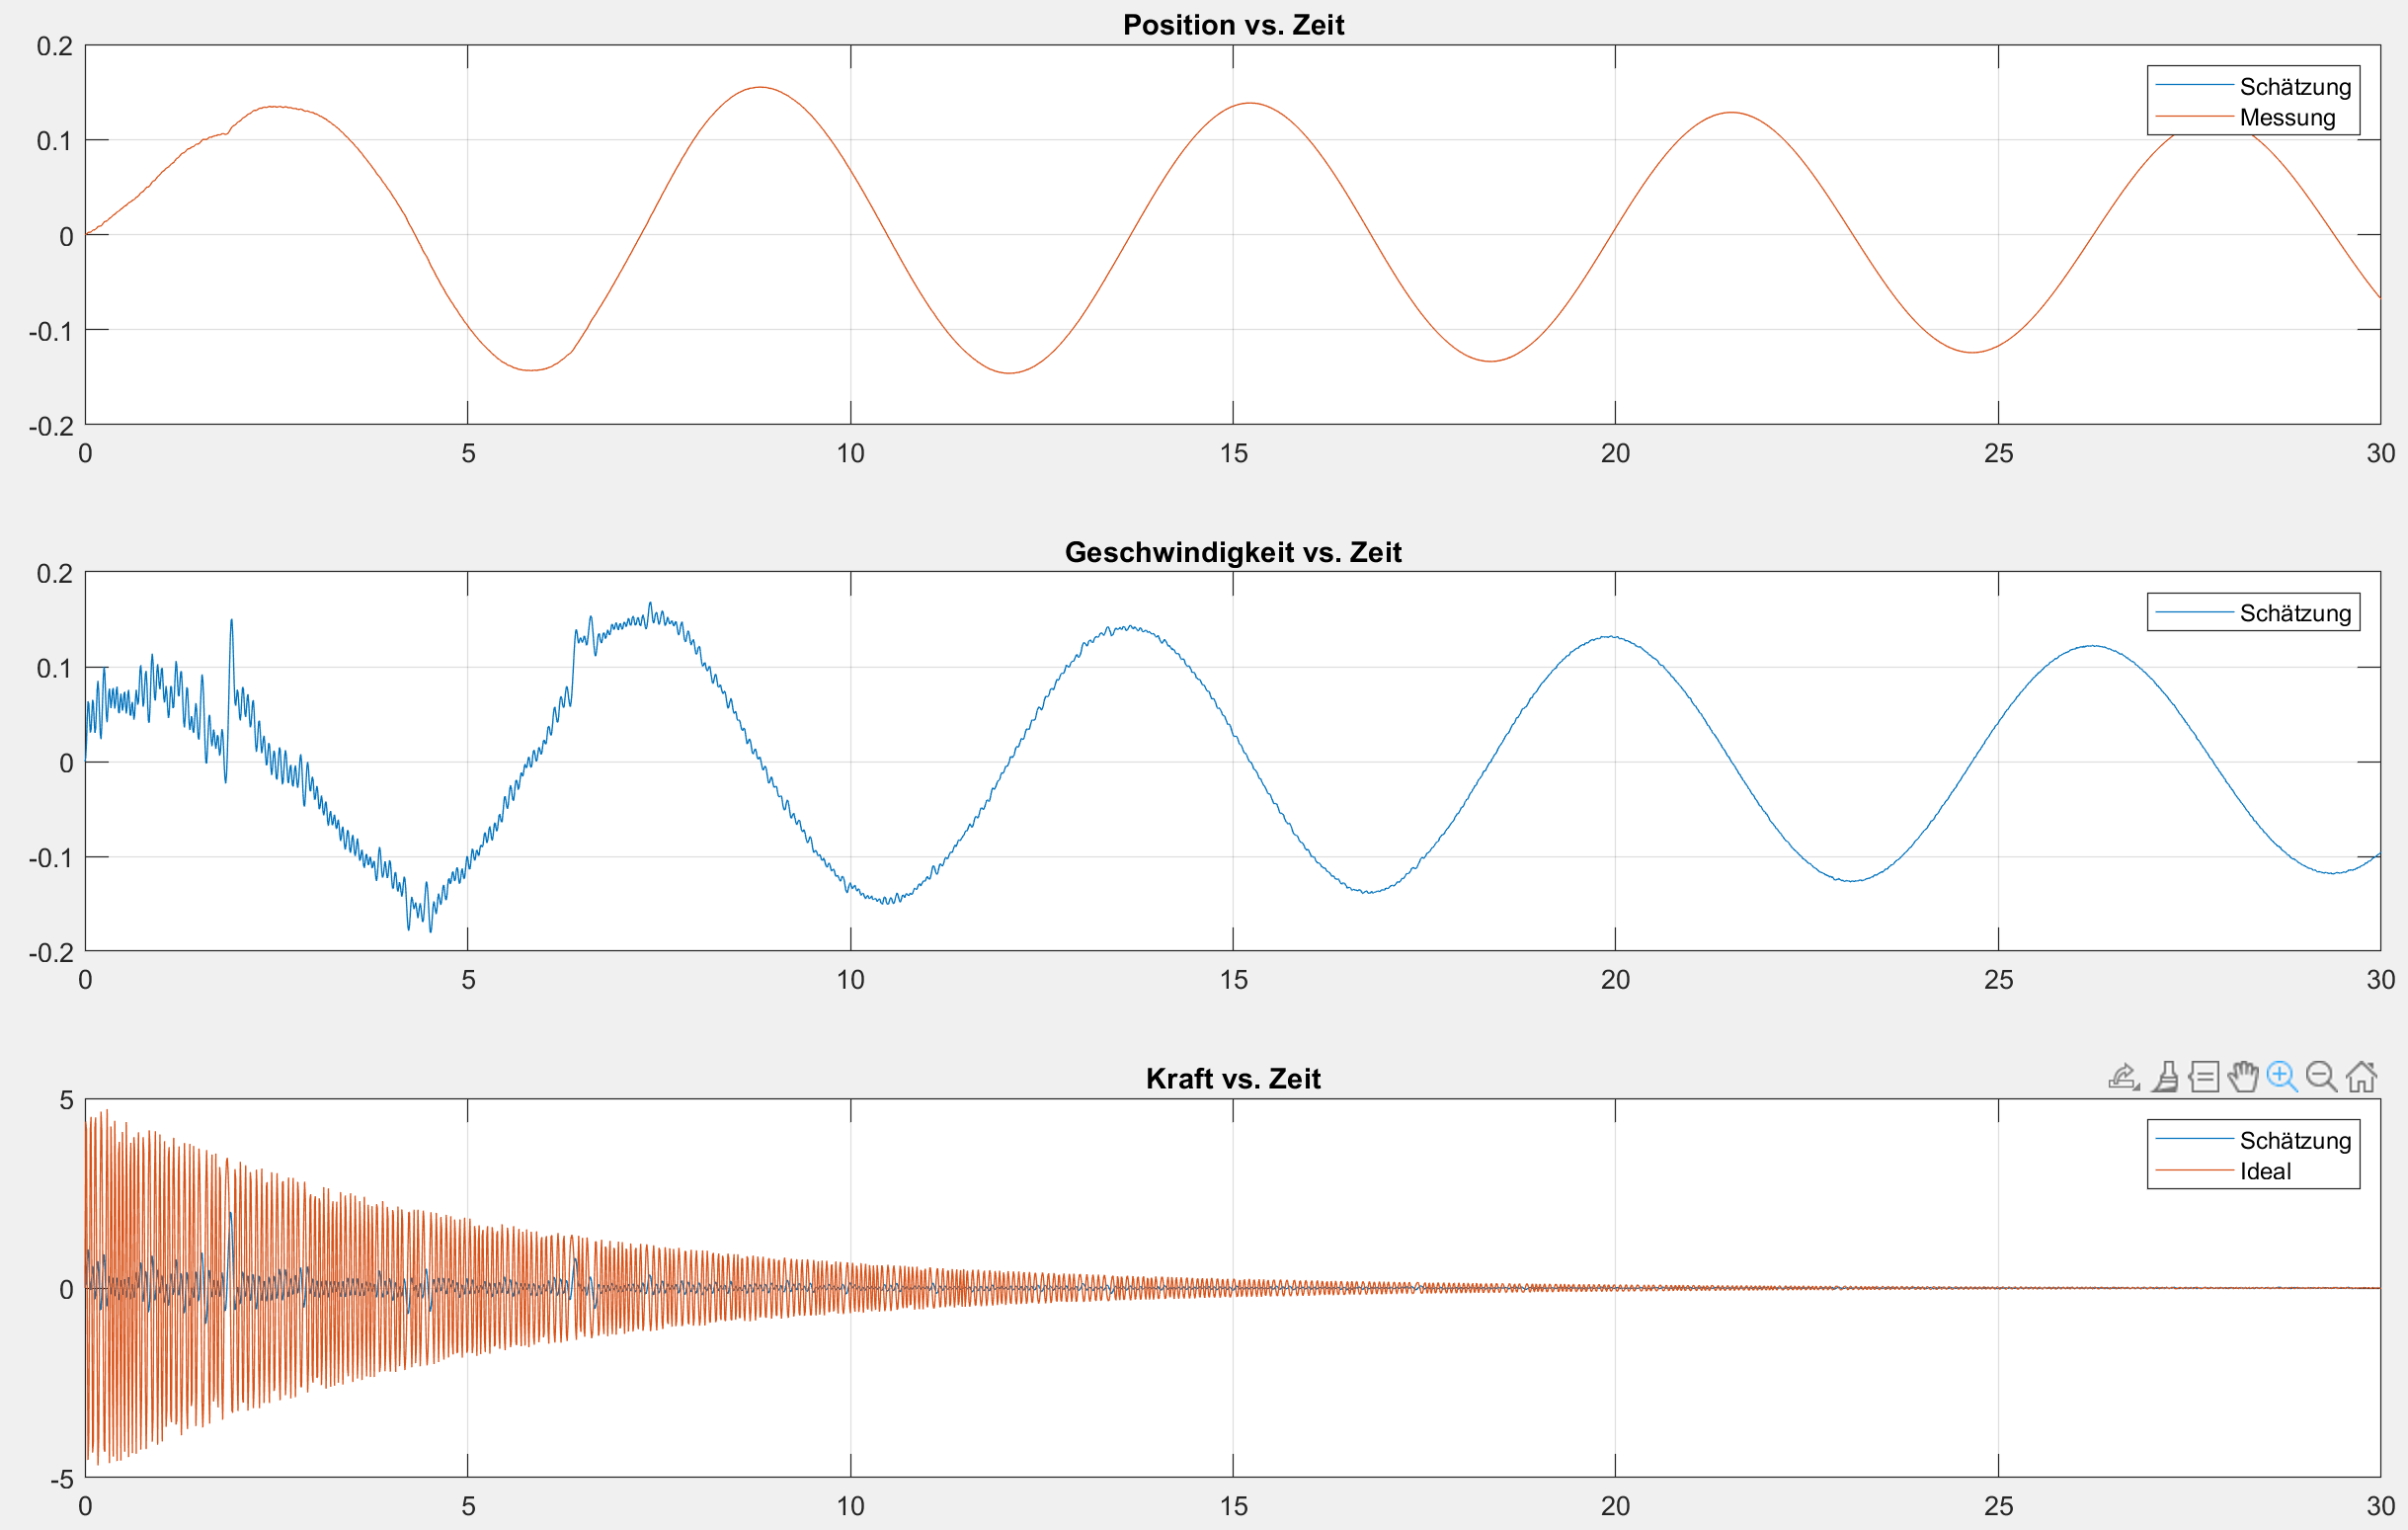
\includegraphics[width=\linewidth,keepaspectratio]{papers/erdbeben/Systemparameter_geaendert.PNG}
      \caption{
        Im Geschwindigkeits-Diagramm erkennen wir,
        dass sich im Vergleich zum Standardfall die Auslenkung und Frequenz vergrössert hat.
        Dies wird mit der Erhöhung der Masse und somit der Trägheit begründet.
        Auch stellen wir fest, dass die Positionsmessung überwiegend die Eigenfrequenz misst.
        Diese wird in der Schätzung der Kraft dennoch sehr gut kompensiert.
      }
    \label{erdbeben:fig:systemparameter-geaendert}
  \end{center}
\end{figure}

\subsection{Verstärkung des Prozessrauschens}
Falls wir unseren Seismographen in der Nähe einer grösseren Stadt aufstellen, so müssen wir aufgrund der Vibrationen mit einem stärkeren Prozessrauschen rechnen.
Dieses Rauschen beeinflusst die Varianzen der Position und Geschwindigkeit in der Matrix $Q$.
Aus diesem Grund erhöhen wir die Standardabweichungen der Positions $\sigma_s$ und Geschwindigkeit $\sigma_v$ in der Matrix $Q$ um den Faktor $100$.
Die Auswertung in Abbildung~\ref{erdbeben:fig:prozessrauschen-geaendert} zeigt auf,
dass das Kalman-Filter die Schätzung der Kraft nur gering an den Messwerten anpasst,
da wir den Schätzungen für die Position nun wenig Vertrauen schenken und stärker der Modell-Annahme $\dot F = 0$ folgen.
Die Theorie dazu haben wir im Abschnitt~\ref{erdbeben:Wahrscheindlichkeit} angeschaut.

\begin{figure}
  \begin{center}
    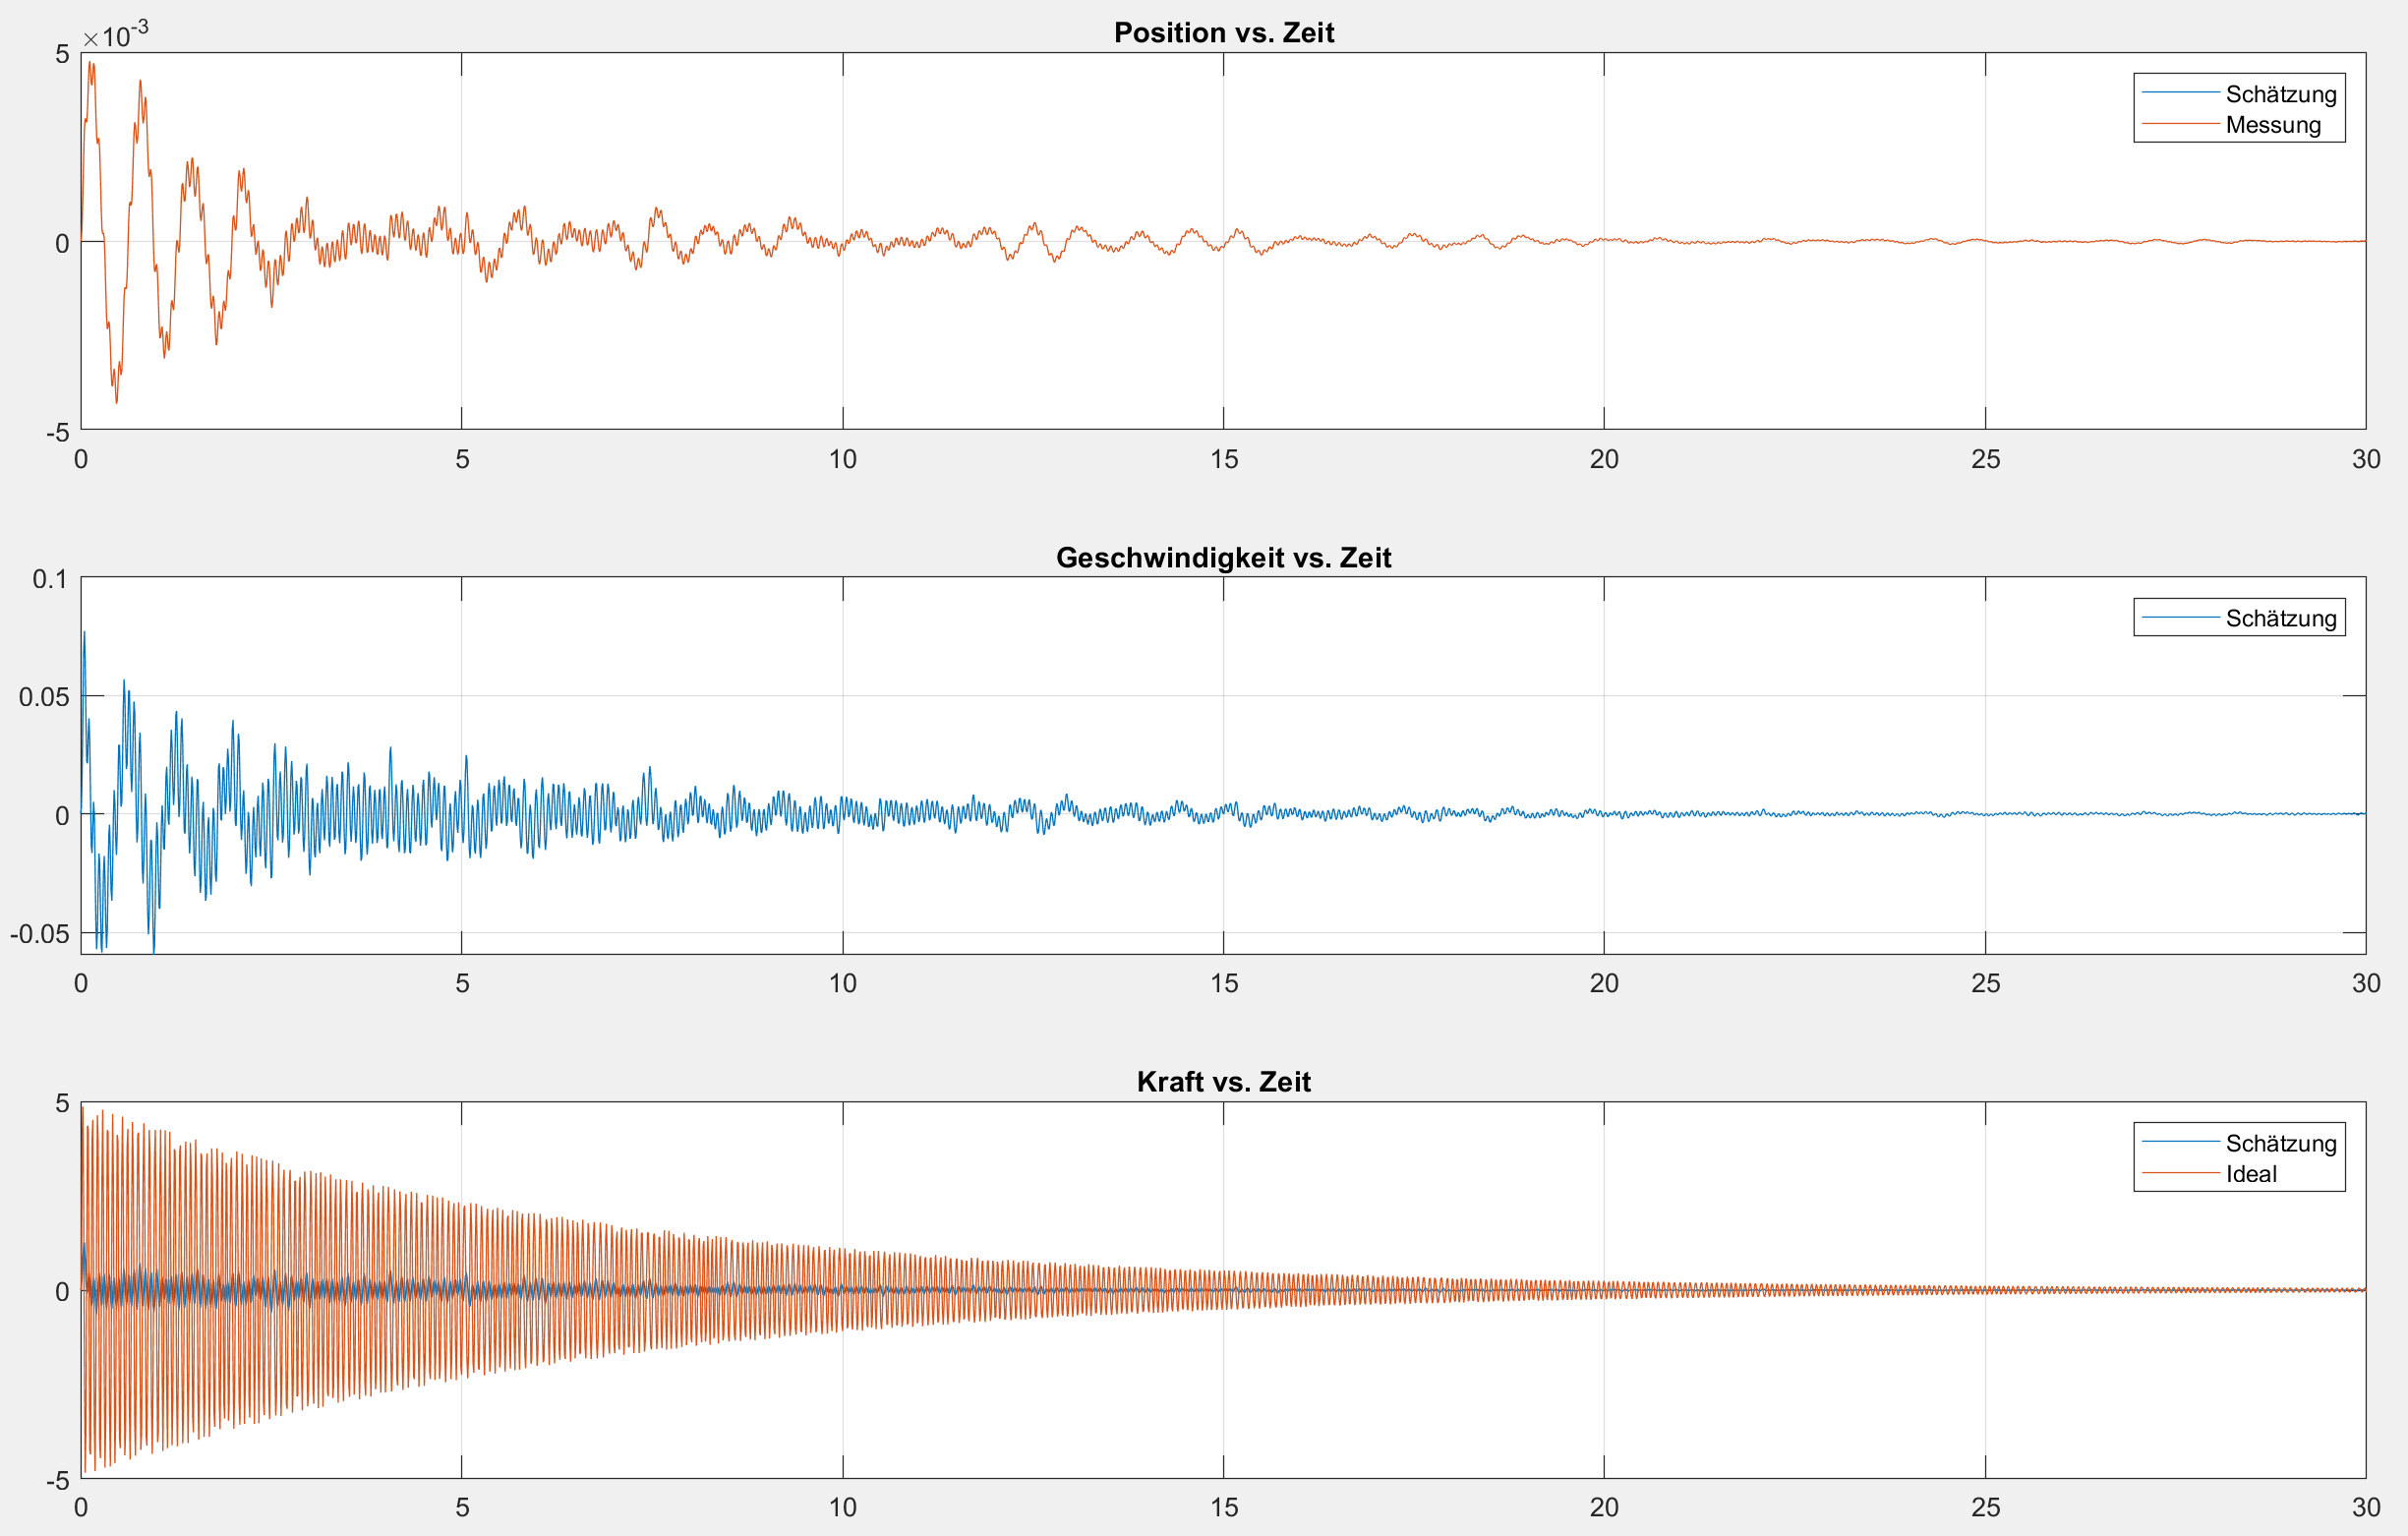
\includegraphics[width=.95\linewidth,keepaspectratio]{papers/erdbeben/images/Prozessrauschen_geaendert.PDF}
    \caption{
      Mit dem Erhöhen des Prozessrauschens gehen wir von einer grösseren Unsicherheit der Systemmatrix aus.
      Aus diesem Grund folgt das Filter vor allem den Messwerten,
      was sichtbare Folgen für die Schätzkurve im Kraft-Zeit-Diagramm hat.
      Hier möchte das Filter auch den Messwerten folgen.
      Da wir aber für die Kraft keine Messwerte aufzeichnen,
      erhalten wir eine sehr schwache Kurve.
      Die Position kann immernoch präzise geschätzt werden und die Ableitung zur Geschwindigkeit ergibt gute Resultate.
      Jedoch ist die Schätzkurve der Kraft sehr weit von der idealen Kurve entfernt und nicht nutzbar.
    }
    \label{erdbeben:fig:prozessrauschen-geaendert}
  \end{center}
\end{figure}

\subsection{Verstärkung des Messrauschens}
Als letztes verstärken wir das Messrauschen um den Faktor $100$ und belassen wieder den Rest wie im Standardfall.
Wie man eigentlich schon erwarten kann,
zeigt uns die Abbildung~\ref{erdbeben:fig:messrauschen-geaendert},
dass das Signal des Messsensors vom Messrauschen start gestört wird.
Weil die Messung zu ungenau ist,
kann das Kalman-Filter nicht mehr gut arbeiten und produziert einen ungenauen Output.

\begin{figure}
  \begin{center}
    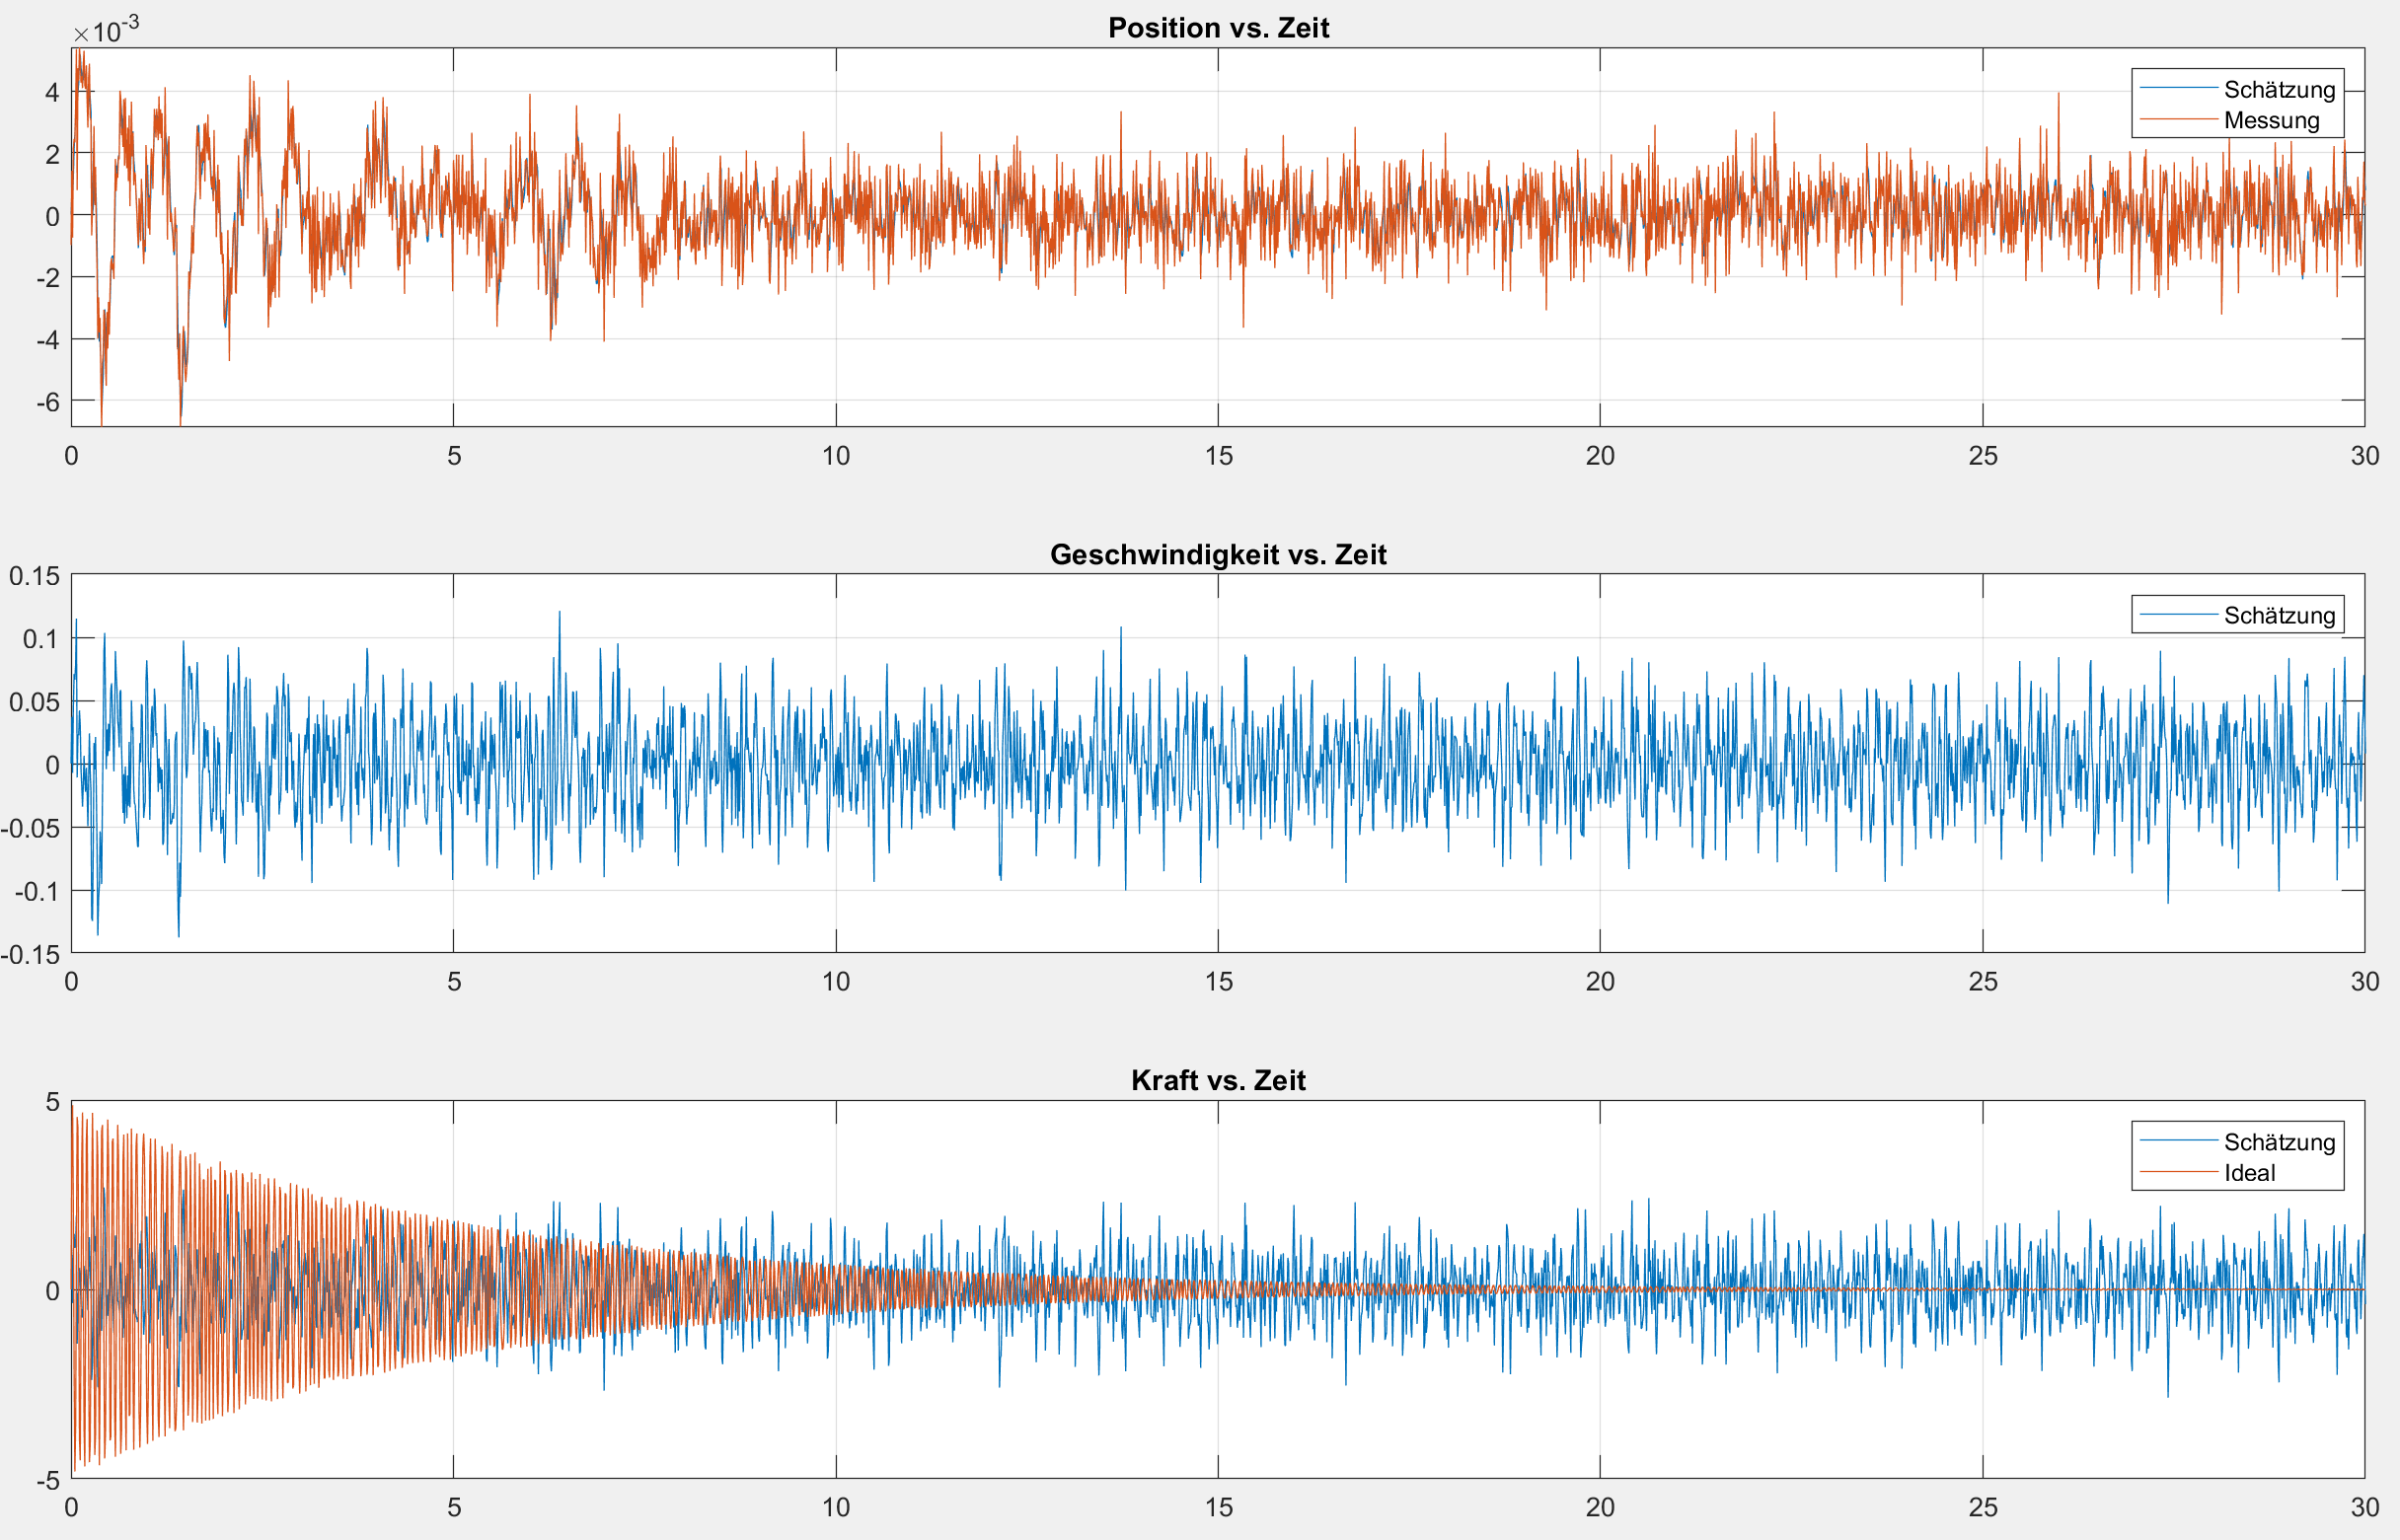
\includegraphics[width=.95\linewidth,keepaspectratio]{papers/erdbeben/images/Messrauschen_geaendert.PDF}
    \caption{
      Im Kraft-Zeit-Diagramm erhalten wir nur bis ca.\ $t = 10$ gute Schätzwerte.
      Ab $t = 10$ wirkt das Messrauschen zu stark und wir erhalten keine brauchbaren Werte mehr.
      Im Position-Zeit-Diagramm erhielten wir bis jetzt immer genaue Schätzungen.
      Mit einem starken Messrauschen fällt es dem Filter nun schwerer,
      präzise Schätzungen zu berechnen.
      Die Nahaufnahme im Kraft-Zeit-Diagramm bestätigt uns,
      dass die Messfehler zu gross sind,
      um ein klares Bild über die äussere Kraft zu erhalten.
    }
   \label{erdbeben:fig:messrauschen-geaendert}
  \end{center}
\end{figure}

\subsection{Zusammenfassung}
Wir haben uns zum Ziel gesetzt,
die äussere Beschleunigung $a(t)$,
beziehungsweise die Kraft $f(t)$ eines Erdbebens
aus den Messugnen eines Seismographen zu berechen.

Wir haben einen Seismographen mathematisch beschrieben und
mit der Software Matlab Messresultate während eines künstlichen Erdbebens erzeugt.
Diese Messwerte haben wir mit einem Kalman-Filter bearbeitet,
um aus den Messwerten wieder das Erdbeben zu gewinnen.

Der Seismograph war fähig, die Position der Masse während der Einwirkung des Erdbebens aufzuzeichnen.
$a(t)$ kann zwar nicht mit Sensoren gemessen werden, jedoch erhalten wir $a(t)$ durch zweifaches Ableiten.
Da wir so aber die innere Beschleunigung erhalten, mussten wir das Kalman-Filter anwenden.
Das Kalman-Filter half uns, die äussere Beschleunigung zu schätzen, und lieferte erstaunlich genaue Werte.
Ausserdem hat es das Filter geschafft, die Eigenfrequenz der Masse und die Erdbebenfrequenz zu separieren.
Folglich erhielten wir eine Schätzung, die nur das Erdbeben betraf.

Zuletzt haben wir aufgezeigt,
dass Veränderungen an den System- und Rauschparametern die Genauigkeit und Zuverlässigkeit
des Kalman-Filters beeinträchtigen können.
Wir haben gesehen, dass aus zu schlechten Sensordaten auch mittels Filterung keine genauen Aussagen möglich sind.

